\section{Exercício 2 -- Introdução ao Pytorch Convnet}

\begin{itemize}
	\item Notebook: \textit{introducing-pytorch-convnet.ipynb}
\end{itemize}

\subsection{Descrição}

O notebook em questão contém uma série de demonstrações de conceitos básicos do Pytorch, como as operações de convolução, a função de ativação, \textit{pooling}. Além de \textit{skip connections}, camadas densamente conectadas, \textit{dropout} etc. Por fim, há um processo de construção e treinamento de uma rede neural, desde sua construção, definição de função de perda e otimizador, processo de treinamento e validação.

O problema do processo que foi realizado é que houve \textit{overfitting} (Figura~\ref{fig:note2:init_train}), noticiado pelo custo de treinamento consistentemente menor do que o de validação. O exercício em questão consiste numa exploração dos elementos e hiperparâmetros utilizados para melhorar o resultado obtido

\begin{figure}[!htb]
	\centering
	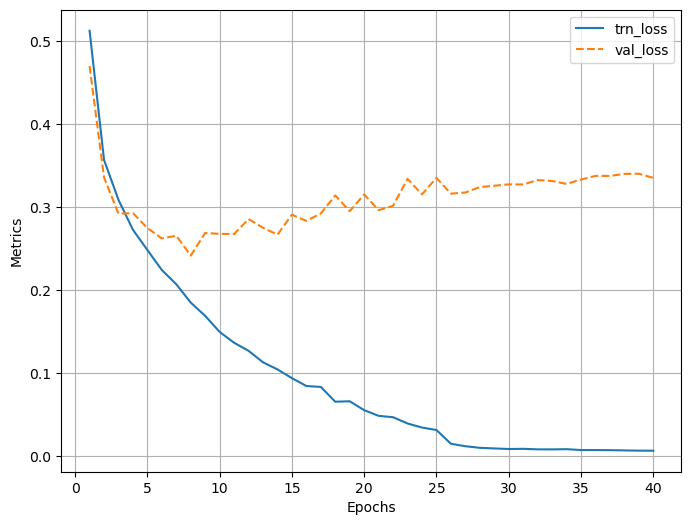
\includegraphics[width=0.6\linewidth]{intro_convnet/initial_train}
	\caption{Gráfico do custo de treinamento e de validação ao longo das épocas de treinamento.}
	\label{fig:note2:init_train}
\end{figure}

\subsection{Resolução do Exercício Proposto}

Além do problema evidenciado na descrição do problema, outro problema noticiado é a instabilidade dos custos, que tem oscilado 